\section{Introduction}

La structure de ce document et certaines parties sont inspir˜es de
\cite{guide}.

L'objectif de ce guide est de donner un cadre ˜ l'˜criture de rapports 
de projet
˜ l'\gls{enstab}.
Il vient compl˜ter le document d'aide ˜ la
r˜daction du rapport de stage op˜rateur \og{}Consignes pour la r˜daction d'un
m˜moire\fg{} disponible sur moodle ˜ l'adresse 
\url{https://moodle.ensta-bretagne.fr/course/view.php?id=408} (section 4). 


La section \ref{sec:gen} pr˜sente les g˜n˜ralit˜s sur la nature d'un rapport
de projet. La section \ref{sec:struct} d˜crit la structure attendue d'un rapport de
projet.
Puis, la section \ref{sec:regles} d˜crit les r˜gles m˜thodologiques et
typographiques ˜ respecter lors de la r˜daction.
Enfin, la section
\ref{sec:outils} offre un aper˜u des outils contribuant ˜ l'˜criture d'un rapport.


\section{G˜n˜ralit˜s}
\label{sec:gen}

En r˜digeant un rapport, vous laissez une trace de votre travail, qui restera
disponible sur le long terme. Il faudra donc veiller ˜ la qualit˜ du fond
comme de la forme.

Afin d'˜tre largement compris, le rapport doit privil˜gier une
˜criture simple (mais non simpliste) faite de phrases courtes,
employant un vocabulaire explicite. Tous les acronymes doivent ˜tre explicit˜s
et tous les termes techniques expliqu˜s.

L'orthographe contribue ˜ l'image que vous laissez de vous-m˜me. Si les
correcteurs orthographiques sont d'un usage indispensable, ils ne remplacent
jamais une relecture soigneuse.
De plus, les usages typographiques de la langue employ˜e doivent ˜tre respect˜s.

Avant l'entamer la r˜daction d'un rapport, les r˜ponses ˜ quelques questions
fondamentales sur le rapport vous permettront de cadrer votre travail.

\subsection*{Pourquoi ?}

La r˜ponse ˜ cette question permet de d˜finir la longueur du
document et son style, et bien entendu la nature du contenu.

\subsection*{Pour qui ?}

La r˜ponse ˜ cette question permet de d˜finir la teneur des propos, les
notions que le lecteur ma˜trise et celles qu'il faut d˜tailler. Elle permet
˜galement de cibler l'analyse ˜ effectuer. Dans certains cas, elle permet
˜galement de fixer le degr˜ de confidentialit˜ et
les modalit˜s de diffusion.

\subsection*{Pour quand ?}

Cette r˜ponse vous permet de g˜rer votre temps. Attention, l'˜criture de
certaines parties n˜cessite un travail de recherche ou d'analyse pr˜alable. De
plus, vous 
pouvez avoir ˜ collecter des informations aupr˜s de tiers dont vous ne
ma˜trisez pas toujours les contraintes.

\subsection*{Pour combien de temps ?}

En r˜pondant ˜ cette question, vous allez d˜finir la dur˜e
d'utilisation du document~; vous en d˜duirez l'utilit˜ d'en g˜rer des versions
cons˜cutives.


\section{Structure du rapport}
\label{sec:struct}

Il n'y a pas de forme unique et universelle pour un rapport.
N˜anmoins, la structure devra toujours comporter des ˜l˜ments qui en
permettent l'utilisation efficace.\index{Structure (rapport)}
Dans tous les cas le rapport devra ˜tre pagin˜ et le texte justifi˜.

 Le rapport devra \emph{obligatoirement} contenir~:
 \begin{itemize}
 \item un r˜sum˜~; 
 \item une page titre~;
 \item une table des mati˜res~;
 \item une introduction~;
 \item un d˜veloppement~; 
 \item une conclusion~;
\item une bibliographie.
 \end{itemize}

%et \emph{pratiquement syst˜matiquement}~:
%\begin{itemize}
%\end{itemize}

\emph{Dans la plupart des cas}, on trouvera  ˜galement~:
\begin{itemize}
\item une liste de mots-cl˜s~;  
\item une table des figures ou illustrations~;
\item des remerciements~;
\item une ou plusieurs annexes.
\end{itemize}

\emph{Dans certains cas}, il contiendra enfin~:
\begin{itemize}
\item un index~;
\item un glossaire.
\end{itemize}

Voyons les caract˜ristiques de ces diff˜rents ˜l˜ments.

\subsection{Page de titre}

La page de titre doit permettre d'identifier le document. Pour cela, elle doit
comprendre~: \index{Page de garde}
\begin{itemize}
\item un titre~;
\item le type du document (par exemple \og{}Rapport de projet\fg{})~;
\item le nom du ou des auteurs du document~;
\item la date de parution (ou de remise du rapport) et ˜ventuellement le
  num˜ro de version~;
\item le nom et le logo de l'organisme dont est issu l'auteur (par exemple
  \textsc{Ensta} Bretagne).
\end{itemize}

\subsection{R˜sum˜}

Le r˜sum˜ fait la synth˜se du projet en une page au maximum. Il
devra contenir une br˜ve description du probl˜me et des objectifs du projet,
mentionner les r˜sultats les plus
importants et dresser une conclusion. Dans le r˜sum˜ il faut surtout mettre en
˜vidence les r˜sultats car ce sont eux qui rendent mieux compte de votre
travail et donnent l'envie de lire votre rapport. 

Le r˜sum˜ est souvent accompagn˜ de quelques mots-cl˜s et il est, dans
certains cas, traduit en une ou plusieurs langues.\index{Resume@R˜sum˜}

\subsection{Table des mati˜res}

Encore baptis˜e \og{} sommaire \fg{}, la table des mati˜res permet de
synth˜tiser, en d˜but de document, les diff˜rents chapitres qui y sont
trait˜s. Elle doit faire
r˜f˜rence ˜ la pagination du document pour permettre au lecteur
d'acc˜der directement ˜ toute partie du document.\index{Table des
  matieres@Table des mati˜res}\index{Sommaire} 

La table des mati˜res se g˜n˜re automatiquement ; ne la cr˜ez pas
manuellement, car vous pourriez oublier d'y apporter des
modifications.

\subsection{Introduction}

L'introduction doit permettre de situer le contexte de votre travail. En
particulier, elle doit~:\index{Introduction}
\begin{itemize}
\item pr˜senter le contexte de l'˜tude~;
\item d˜finir le probl˜me que le projet cherche ˜ r˜soudre, ainsi
    que le cadre dans lequel il s'inscrit~; 
\item d˜finir le cadre du travail ; par exemple quelles ont ˜t˜ les
  contraintes, la m˜thodologie choisie~;
\item annoncer le plan, qui n'est pas un ennonc˜ plat des diff˜rentes parties,
  mais qui vise ˜ d˜finir l'orientation de la recherche, les hypoth˜ses, le
  cheminement choisi pour tenter de r˜pondre ˜ la question.
\end{itemize}

%Il est ˜galement souhaitable de pr˜senter les diff˜rentes parties et leur
%encha˜nement.

\subsection{D˜veloppement}

Le d˜veloppement est la partie substantielle de votre document. Il doit ˜tre
structur˜ et d˜coup˜ en plusieurs parties. Les encha˜nements entre les parties
doivent ˜tre fluides (par exemple gr˜ce ˜ une courte introduction en d˜but de
partie et un court bilan ˜ la fin). Il peut s'appuyer sur des compl˜ments
d'information (notes de bas de page, r˜f˜rences, annexes, glossaires ou listes
d'acronymes). N'h˜sitez pas ˜ illustrer vos propos par des figures, tables
ou ˜quations.

\subsubsection{Notes de bas de page}

Les notes de bas de page servent ˜ apporter un compl˜ment d'information
non essentiel. Le texte doit pouvoir ˜tre compris sans y faire appel.
Elles sont tr˜s utiles lorsque l'on veut que le document puisse avoir
plusieurs niveaux de lecture.\index{Notes de bas de page}

\subsubsection{Figures et graphiques}

Si on se r˜f˜re ˜ \cite{tufte}, les graphiques de qualit˜ doivent
communiquer au lecteur un maximum d'information en un minimum de temps. Lors
de l'utilisation de figures, vous vous attacherez ˜ respecter les r˜gles
suivantes~:\index{Figures}
\begin{itemize}
\item Toutes les figures doivent poss˜der un titre et ˜tre cit˜es dans le
  document (par exemple \og{}la figure \ref{fig:fract} nous montre que
  \ldots{}\fg{})~; la num˜rotation des figures doit ˜tre g˜r˜e
  automatiquement.
\item La mise en page doit ˜tre homog˜ne ˜ l'int˜rieur d'un graphique.
\item Des graphiques s˜par˜s servant de base ˜ des comparaisons doivent avoir
  une mise en page coh˜rente. Ils doivent notamment ˜tre repr˜sent˜s ˜ la m˜me
  ˜chelle et utiliser la m˜me palette de couleurs.
\item Selon \cite{tufte}, pour de petits ensembles de
  donn˜es\footnote{moins de 20 donn˜es}, les 
  tableaux sont plus informatifs que les graphiques.
\item Les graphiques doivent ˜tre correctement ˜tiquet˜s~:
  \begin{itemize}
  \item si $x$ repr˜sente les abscisses et $y$ les ordonn˜es, faites en sorte
    que $y=f(x)$ plut˜t que $x=f(y)$~;
  \item n'oubliez pas les unit˜s sur les axes, typiquement entre crochets
    (voir figure \ref{fig:fract}).
  \end{itemize}
\item Chaque graphique doit ˜tre analys˜ dans le corps du document.
\end{itemize}

\begin{figure}[htbp]
  \centering
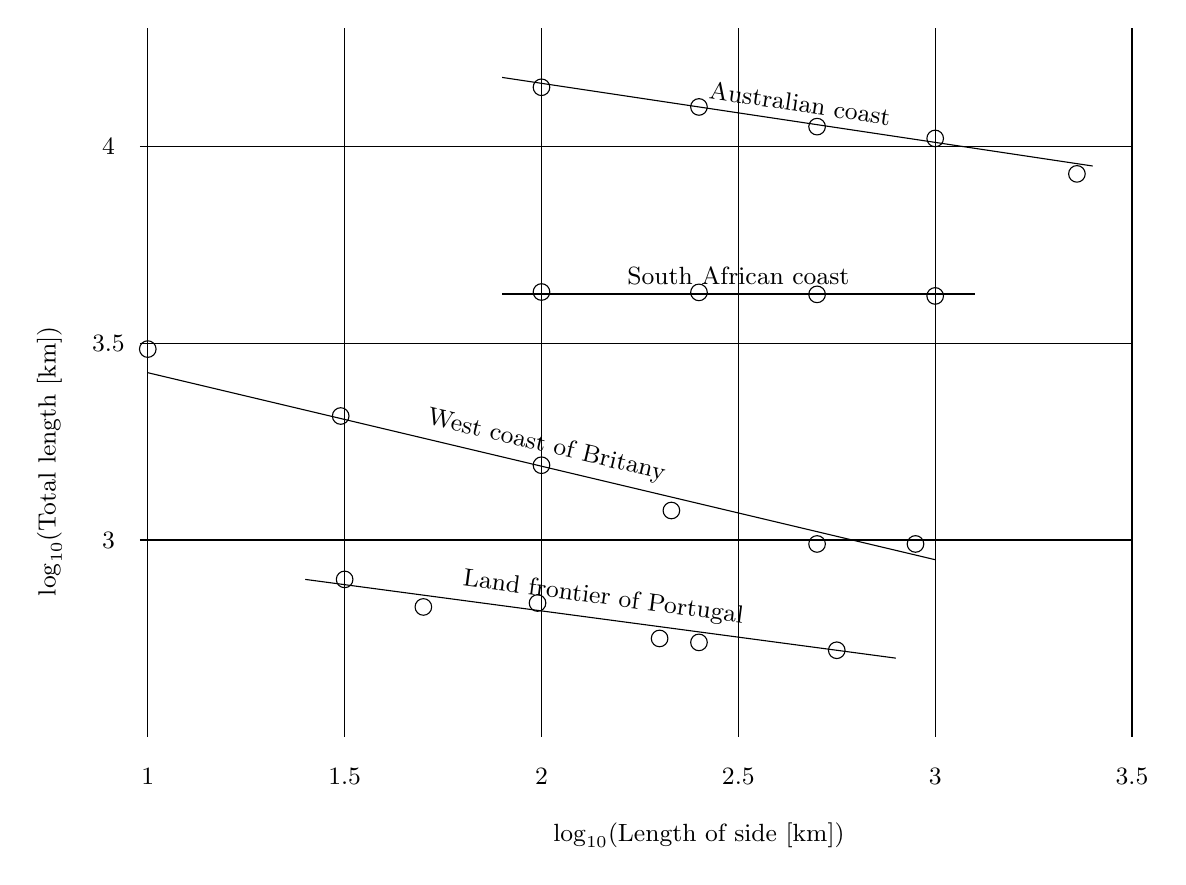
\begin{tikzpicture}[x=1cm,y=1cm,scale=5,font=\small]
  \draw[step=0.5] (0.98,2.5) grid (3.5,4.3);
  \foreach \x/\y in {1/3.485,1.49/3.315,2/3.19,2.33/3.075,2.7/2.99,2.95/2.99,1.5/2.9,1.7/2.83,1.99/2.84,2.3/2.75,2.4/2.74,2.75/2.72,2/3.63,2.4/3.629,2.7/3.624,3/3.62,2/4.15,2.4/4.1,2.7/4.05,3/4.02,3.36/3.93} {
    \draw (\x,\y) circle (0.6pt);
  }
  \draw (1,3.425) -- node[sloped, above] {West coast of Britany}
  (3,2.95);
  \draw (1.4,2.9)-- node[sloped, above] {Land frontier of Portugal} (2.9,2.7);
  \draw (1.9,3.625)-- node[sloped, above] {South African coast} (3.1,3.625);
  \draw (1.9,4.175)-- node[sloped, above] {Australian coast} (3.4,3.95);
  \foreach \x in {1,1.5,...,3.5} {
    \draw (\x,2.4) node {\x};
  }
  \node at (2.4,2.25) {$\log_{10}$(Length of side [km])};
  \foreach \y in {3,3.5,4} {
    \draw (0.9,\y) node {\y};
  }
  \node[rotate=90] at (0.75,3.2) {$\log_{10}$(Total length [km])};
\end{tikzpicture}
  \caption{Dimension fractale de traits de c˜te de diff˜rents pays ; relation entre longueur et pas}
  \label{fig:fract}
\end{figure}

De mani˜re g˜n˜rale, prenez garde ˜ la lisibilit˜ de vos figures. Pensez
˜galement que la lisibilit˜ est diff˜rente sur ˜cran, sur une impression
couleur, ou sur une impression en noir et blanc.

Concernant le format des figures, pr˜f˜rez dans la mesure du possible les
formats vectoriels\footnote{qui ne se d˜gradent pas lors des changements de
  taille} comme \emph{eps}, \emph{pdf} ou \emph{svg}. Si vous optez pour un
format image sachez que, de part son algorithme de compression, le format
\emph{jpg} d˜gradera fortement le texte~; pr˜f˜rez-lui le format \emph{png}.

Dans le cas o˜ la figure est issue d'une capture d'˜cran, pensez ˜ ajouter un
habillage et gardez toujours ˜ l'esprit la lisibilit˜ de la figure~; si
n˜cessaire, modifiez les couleurs dans un outil de traitement
d'images\footnote{Par exemple \textsc{gimp}}. 

\subsubsection{Tables}

De la m˜me mani˜re que les figures, les tables servent ˜ illustrer certains
˜l˜ments du rapport. Elles doivent poss˜der un titre et ˜tre
r˜f˜renc˜es dans le corps du document. Il faut prendre garde ˜ leur
lisibilit˜. Un exemple \emph{˜ ne pas suivre} est pr˜sent˜ table
\ref{tab:tab1} (table extraite du manuel de \LaTeX). Dans cet exemple, les
lignes (horizontales et verticales) sont 
trop nombreuses et nuisent ˜ la lisibilit˜, les alignements sont erratiques,
les unit˜s ne sont pas correctement indiqu˜es et les nombres sont repr˜sent˜s
avec des pr˜cisions diff˜rentes. Enfin, les titres de chaque colonne ne sont
pas apparents.\index{Tables}

\begin{table}[htbp]
  \centering
\begin{tabular}{||l|lr||} 
\hline
\hline
~~~~~gnats     & gram      & 013.65\euro \\ \cline{2-3}
          & each      & .01 \\ \hline
gnu       & stuffed   & 92.5 \\ \cline{1-1} \cline{3-3}
~~~emu       &           & 33.33 \\ \hline
armadillo & frozen    & 8.9887 \\ \hline
\end{tabular}
  \caption{Une table tr˜s mal pr˜sent˜e}
  \label{tab:tab1}
\end{table}

La table \ref{tab:tab2} corrige tous les probl˜mes de la table
\ref{tab:tab1}. Cette fois, la table est lisible et elle peut apporter un
compl˜ment d'information au texte.

\begin{table}[htbp]
  \centering
\begin{tabular}{@{}llr@{}} 
  \toprule
  \multicolumn{2}{c}{\textbf{Item}} \\ 
  \cmidrule(r){1-2}
  \textbf{Animal} & \textbf{Description} & \textbf{Price (\euro)}\\ 
  \midrule
  Gnat  & per gram  & 13.65 \\
           & each      & 0.01 \\
      Gnu   & stuffed   & 92.50 \\
      Emu   & stuffed   & 33.33 \\
      Armadillo & frozen & 8.99 \\ 
      \bottomrule
\end{tabular}
  \caption{Une table correctement pr˜sent˜e}
  \label{tab:tab2}
\end{table}

\subsubsection{˜quations}

Il est parfois plus simple de d˜crire un processus par des ˜quations que par
du texte. 
De la m˜me mani˜re que les figures et les tables, les ˜quations
doivent ˜tre num˜rot˜es, et ˜tre r˜f˜renc˜es dans le texte du
rapport. \index{Equations@˜quations}

Exemple~: Soit $S={p_1,\ldots,p_n}$ un ensemble fini de points de
$\nbR^d$. L'˜quation \eqref{eq:1} d˜crit l'enveloppe convexe de $S$.

\begin{equation}
  \label{eq:1}
  \mathcal C(S)=
  \left\{
    \sum_{i=1}^n\alpha_i p_i \mbox{ avec } \forall i, \alpha_i\geqslant 0
    \mbox{ et } \sum_{i=1}^n\alpha_i =  1
  \right\}
\end{equation}

\subsection{Conclusion}

La conclusion est une syth˜se de votre travail et doit en faire un bilan
(critique) vis-˜-vis des 
objectifs initiaux. 
Vous devez ici mentionner vos doutes et certitudes quant ˜
vos r˜sultats~; n'h˜sitez-pas ˜ fournir des pistes pour un travail ˜ venir ou
des explications pour un travail non abouti.

\index{Conclusion}

\emph{Introduction et conclusion sont des parties essentielles d'un
  document. En les lisant, le lecteur doit pouvoir se faire une id˜e
  pr˜cise du contenu d˜velopp˜ dans le corps du texte. Il est
  important d'y apporter le plus grand soin.}

\subsection{Bibliographie}

\paragraph{Remarque~:} ce document ne d˜crit pas la m˜thode
permettant de rechercher des r˜f˜rences bibliographiques. Pour cela,
reportez vous ˜ l'UV 1.4 \og{}Bibliographie\fg{} accessible sur moodle~:
\url{https://moodle.ensta-bretagne.fr/course/view.php?id=617}.

La bibliographie reprend toutes les r˜f˜rences qui ont servi de support lors de
votre travail. Elle ne doit contenir que les r˜f˜rences lues et qui sont
cit˜es dans le corps du document.\index{Bibliographie}

Afin de faciliter la maintenance et l'homog˜n˜it˜ de la bibliographie, il est
conseill˜ de s'appuyer sur un outil de gestion de r˜f˜rences tel que
\emph{Zotero} ou BibTeX. Certains outils\footnote{\emph{Zotero} par exemple,
  mais ˜galement des sites tels que \url{https://www.diigo.com} ou
  \url{http://www.citethisforme.com}}
permettent une gestion collaborative des r˜f˜rences.

Exemple~: \emph{Selon \cite{tufte}, pour de petits ensembles de
  donn˜es, les tableaux sont plus informatifs que les graphiques.}

L'utilisation de r˜f˜rences bibliographiques permet~:
\begin{itemize}
\item d'indiquer les r˜sultats et conclusions qui viennent d'autres
  travaux (ne pas citer ses sources constitue une faute grave)~;
\item de donner plus de force ˜ vos propos en vous appuyant sur des r˜sultats
  reconnus par la communaut˜ scientifique~;
\item de vous affranchir de l'˜criture d'une d˜monstration ou d'un calcul~;
\item de citer les documents techniques sur lesquels vous vous appuyez~;
\item de donner des pistes d'exploration pour ceux qui veulent creuser
  certains points.
\end{itemize}

Il existe plusieurs styles classiques de bibliographie, comme par exemple le
format num˜rot˜ dans lequel les r˜f˜rences sont index˜es par un num˜ro entre
crochets. Les r˜f˜rences sont alors ordonn˜es selon l'ordre d'apparition dans
le document.

\paragraph{Exemple de bibliographie num˜rot˜e~:}
\begingroup
\renewcommand{\section}[2]{}%
\begin{thebibliography}{1}
\bibitem{n1} Rudolf \textsc{Bayer} et Edward Meyers \textsc{McCreight}. ``Organization and
  maintenance of large ordered indexes''. In : \emph{Acta Informatica} 1.3
  (1972), p. 173--189.
\bibitem{n3} Beno˜t \textsc{Mandelbrot}. ``How long is the coast of Britain ?
  Statistical selfsimilarity and fractional dimension''. In: \emph{Science}
  156.3775 (5 mai 1967), p. 636.
\bibitem{n2} Kenneth Lee \textsc{Clarkson} et al. ``Approximating center points with
  iterated Radon points''. In : \emph{International Journal of
    Computational Geometry \& Applications} 06.03 (sept. 1996), p. 357--377.
\end{thebibliography}
\endgroup

~\\
Un autre format classique est le format alphab˜tique dans lequel les
r˜f˜rences apparaissent dans l'ordre alphab˜tique et sont compos˜es de lettres
suivies de deux chiffres repr˜sentant l'ann˜e. Ces lettres sont~:
\begin{itemize}
\item les trois premi˜re lettres du nom de l'auteur (s'il est seul)~;
\item les initiales des auteurs (s'ils sont deux ou trois)~;
\item les trois premi˜re lettres du nom du premier auteur suivies du symbole
  \og{}+\fg{} (s'il y a plus de 3 auteurs).
\end{itemize}

\paragraph{Exemple de bibliographie alphab˜tique~:}
\begingroup
\renewcommand{\section}[2]{}%
\begin{thebibliography}{WWW99}
\bibitem[BM72]{a1} Rudolf \textsc{Bayer} et Edward Meyers \textsc{McCreight}. ``Organization and
  maintenance of large ordered indexes''. In : \emph{Acta Informatica} 1.3
  (1972), p. 173--189.
\bibitem[Cla+99]{a2} Kenneth Lee \textsc{Clarkson} et al. ``Approximating center points with
  iterated Radon points''. In : \emph{International Journal of
    Computational Geometry \& Applications} 06.03 (sept. 1996), p. 357--377.
\bibitem[Man67]{a3} Beno˜t \textsc{Mandelbrot}. ``How long is the coast of Britain ?
  Statistical selfsimilarity and fractional dimension''. In: \emph{Science}
  156.3775 (5 mai 1967), p. 636.
\end{thebibliography}
\endgroup

\subsection{Annexes}

Les annexes regroupent les informations qui ne sont pas essentielles ˜ la
compr˜hension g˜n˜rale du rapport et dont la pr˜sence dans le texte principal
nuirait ˜ la fluidit˜ de la lecture. Les annexes peuvent par exemple
contenir~:\index{Annexes}
\begin{itemize}
\item des d˜monstrations ou des calculs d˜taill˜s~;
\item des donn˜es techniques (de mat˜riel par exemple)~;
\item des donn˜es brutes\footnote{uniquement si leur lecture apporte un
    compl˜ment d'information utile au lecteur.}~;
\item des glossaires et index.
\end{itemize}

\paragraph{Remarque~:} les programmes offrent rarement un int˜r˜t dans les
annexes papier. Par contre, il peut ˜tre int˜ressant de les joindre sous forme
num˜rique\footnote{Par exemple dans un fichier archive \emph{7z}, \emph{tgz},
  \emph{tbz}, \emph{zip} ou \emph{rar}.}.

\subsection{Index et glossaire}

L'index et le glossaire sont plac˜s dans les derni˜res pages du
document. L'index permet de retrouver les termes cl˜s du document par une
recherche alphab˜tique~; il acc˜l˜re la recherche d'information dans les
rapports volumineux.\index{Index}

Le glossaire permet de regrouper la description de termes techniques et de
sigles ˜ la fin du document. Il permet une meilleure compr˜hension des
concepts dont l'explication n'est pas reprise en d˜tail dans le texte.\index{Glossaire}

\section{R˜gles}
\label{sec:regles}

\subsection{R˜gles m˜thodologiques}

Le document doit ˜tre consid˜r˜ comme un tout homog˜ne et non comme
une compilation d'˜l˜ments disparates. Les auteurs sont solidairement
responsables (en contenu et en d˜lai) de la totalit˜ du document et
non uniquement de leur propre contribution.\index{Methodologie@M˜thodologie}

La coh˜rence doit ˜tre recherch˜e ˜ tous les niveaux afin de limiter
les ambigu˜t˜s et d'am˜liorer la qualit˜ du document produit. Avant la remise
d'un rapport cons˜quent, plusieurs phases de relecture sont g˜n˜ralement
n˜cessaires. Il est donc conseill˜ de commencer l'˜criture du rapport d˜s que
possible. 

On veillera tout particuli˜rement ˜~:
\begin{itemize}
\item respecter la coh˜rence du style, des  temps et des modes employ˜s ;
\item conserver le m˜me mode de locuteur dans tout le texte (p.~ex.
  je, nous, l'˜quipe) ;
\item utiliser le m˜me niveau de vocabulaire tout au long du texte. 
\end{itemize}

\subsection{R˜gles de typographie}

Les usages de typographie diff˜rent d'une langue ˜ l'autre. Si le rapport est
˜crit en anglais, vous devez alors respecter les usages
anglo--am˜ricains~; consultez par exemple \cite{typoUS} pour des
informations d˜taill˜es. \index{Typographie}

De m˜me, dans tous les cas o˜ vous ˜crivez votre rapport en
fran˜ais, il est important de respecter les r˜gles de typographie fran˜aise.
Dans ce cas,
la lecture de \cite{andreTypo} vous donnera un tr˜s bon aper˜u des r˜gles
˜ respecter et des ˜cueils ˜ ˜viter.

\subsection{R˜gles de pr˜sentation de r˜sultats num˜riques}

Sauf dans le cas de valeurs dimensionnelles, les unit˜s des r˜sultats
num˜riques doivent toujours ˜tre pr˜cis˜es. 

Il est ˜galement important d'˜tre conscient du sens implicite donn˜ lors de la
pr˜sentation de valeurs num˜riques. En particulier, le nombre de chiffres
significatifs pr˜sent˜ traduit la fid˜lit˜ de la mesure. Les chiffres
significatifs excessifs doivent ˜tre supprim˜s par arrondi.

\section{Outils d'aide ˜ la production de documents}
\label{sec:outils}

Lors de votre scolarit˜ ˜ l'\gls{enstab}, vous avez g˜n˜ralement le
choix des outils utilis˜s pour la production de documents. 

\subsection{Traitement de texte et formateur de texte}

Un traitement de texte est un outil de mise en page de documents. Il est
g˜n˜ralement de type \gls{wysiwyg}\footnote{What You See Is What You Get}
et permet donc de voir l'aspect du document se modifier en continu. Dans cette
cat˜gorie, les outils les plus connus sont \emph{Microsoft Word} et
\emph{LibreOffice}. Le formatage du texte est
obtenu par application de {\em styles}. Malheureusement, de nombreux
utilisateurs, insuffisamment form˜s, n'utilisent pas ou utilisent mal
cette fonctionnalit˜.

Le formateur de texte le plus connu est \LaTeX. Il proc˜de en s˜parant le fond
et la forme du document et poss˜de des biblioth˜ques de style qui permettent
de respecter les r˜gles typographiques. Cet outil est g˜n˜ralement
non-\gls{wysiwyg} et requiert un certain investissement avant d'˜tre
utilis˜ efficacement.

\subsection{Format des donn˜es}

La question du format de donn˜es se pose obligatoirement lors de la
manipulation de documents num˜riques. Le choix du format est souvent li˜ ˜
l'outil utilis˜. Dans la mesure du possible, il est conseill˜ d'utiliser des
formats ouverts (c'est-˜-dire dont la sp˜cification est disponible).
Cette question est particuli˜rement importante lors du partage de document.

Voici quelques conseils pour vous aider dans le choix du format de donn˜es~:
\begin{itemize}
\item lors de la remise de documents \emph{non modifiables}, destin˜s ˜ des
  sorties papier, il est conseill˜ d'utiliser le format \emph{pdf}~; soyez
  vigilants ˜ l'int˜gration des polices de caract˜res lors de la g˜n˜ration et
  v˜rifiez syst˜matiquement le r˜sultat~; 
\item pour des documents consultables en ligne, le format \textsc{Html}
  conviendra parfaitement~;
\item pour l'˜change de documents ˜ modifier, les formats \emph{odt},
  \emph{rtf} et \emph{tex} sont ouverts~;
\item en ce qui concerne le format \emph{docx}, les sp˜cifications existent,
  mais ne sont pas exactement respect˜es par \emph{Microsoft Word}, ce qui
  entra˜ne des probl˜mes de mise en page lors du passage par
  \emph{LibreOffice}\ldots{} Dans ce cas, il faudra veiller ˜ ce que tous les
  r˜dacteurs utilisent la m˜me version de \emph{Microsoft Word} ou de
  \emph{LibreOffice}. 
\end{itemize}

\subsection{Outils collaboratifs}

R˜diger un rapport ˜ plusieurs est toujours une op˜ration
d˜licate. L'utilisation d'outils collaboratifs permet de simplifier cette
phase, de manipuler plusieurs versions du document et de g˜rer les conflits.
Plusieurs solutions sont disponibles~:
\begin{itemize}
\item utiliser le mode \og{}Modifications\fg{} de \emph{Microsoft Word} ou de
  \emph{LibreOffice}~; l'˜change de fichiers et la gestion de version doivent
  alors ˜tre assur˜s manuellement~;
\item utiliser un gestionnaire de version\footnote{Par exemple du \textsc{cvs}
  ou du \emph{subversion} h˜berg˜ sur le serveur
  \url{https://gforge.ensta-bretagne.fr/gf} ou une gestion d˜centralis˜e avec
  \url{https://github.com}.} pour h˜berger le code source
\LaTeX\footnote{Cette m˜thode ne fonctionne que si le document est au format
  texte.}~;
\item h˜berger le rapport sur un service \emph{cloud} tel que
  \emph{Google drive} ou \emph{Microsoft Office 365}.
\end{itemize}

\section{Conclusion}

Dans ce guide, les objectifs d'un rapport de projet ont
˜t˜ pr˜cis˜s ainsi que la structure classique de son plan. Ensuite,
les r˜gles de base pour sa r˜daction ont ˜t˜ pr˜sent˜es, suivies d'un
rapide traitement des probl˜matiques li˜es aux outils de production de
documents. 



%%% Local Variables: 
%%% mode: latex
%%% TeX-master: "../guide"
%%% End: 
